% -*- Mode:TeX -*-

%% IMPORTANT: The official thesis specifications are available at:
%%            http://libraries.mit.edu/archives/thesis-specs/
%%
%%            Please verify your thesis' formatting and copyright
%%            assignment before submission.  If you notice any
%%            discrepancies between these templates and the 
%%            MIT Libraries' specs, please let us know
%%            by e-mailing thesis@mit.edu

%% The documentclass options along with the pagestyle can be used to generate
%% a technical report, a draft copy, or a regular thesis.  You may need to
%% re-specify the pagestyle after you \include  cover.tex.  For more
%% information, see the first few lines of mitthesis.cls. 

%\documentclass[12pt,vi,twoside]{mitthesis}
%%
%%  If you want your thesis copyright to you instead of MIT, use the
%%  ``vi'' option, as above.
%%
%\documentclass[12pt,twoside,leftblank]{mitthesis}
%%
%% If you want blank pages before new chapters to be labelled ``This
%% Page Intentionally Left Blank'', use the ``leftblank'' option, as
%% above. 

\documentclass[12pt,twoside]{mitthesis}
\usepackage[spanish,es-tabla,es-noquoting]{babel} % Idioma y codificación del texto
\usepackage[utf8x]{inputenc} % Codificación del archivo
\usepackage{hyperref}
\hypersetup{%
    colorlinks=true
}
\usepackage{tikz}
\usepackage{pgfplots}
\pgfplotsset{%
    /pgf/number format/use comma,
    /pgf/number format/set thousands separator = {},
}
\usepackage[justification=centering]{caption}
\usepackage{framed}
\usepackage{caption}
\usepackage{subcaption}
\usepackage{tabu}
\usepackage{fancyvrb}
\usepackage{listings}
%\usepackage{draftwatermark}
%\SetWatermarkText{DRAFT}
%\SetWatermarkScale{5}
%\SetWatermarkColor[rgb]{0.97,0.97,0.97}


%% La tipografía tiene que soportar tildes, no todas lo hacen %%
\usepackage{courier}    % Courier para tipografía monoespaciada
\usepackage{lmodern}
\usepackage[T1]{fontenc}
 
%% Si se usa hyperref + utf8x para establecer el título, autor, etc... %%
\PrerenderUnicode{á}
\PrerenderUnicode{é}
\PrerenderUnicode{í}
\PrerenderUnicode{ó}
\PrerenderUnicode{ú}
\PrerenderUnicode{ñ}

%% Los listings precisan parámetros especiales, sino puede fallar la generación del PDF %%
\lstset{
    numbers=left,
    captionpos=b,
    basicstyle=\ttfamily\footnotesize,
    extendedchars=true,
    inputencoding=utf8x,
    literate={á}{{\'a}}1
          {é}{{\'e}}1
          {í}{{\'i}}1
          {ó}{{\'o}}1
          {ú}{{\'u}}1
          {ñ}{{\~n}}1
}
\renewcommand{\lstlistingname}{Código}
\renewcommand\lstlistlistingname{Índice de códigos}

\usepackage{lgrind}
%% These have been added at the request of the MIT Libraries, because
%% some PDF conversions mess up the ligatures.  -LB, 1/22/2014
\usepackage{cmap}
\usepackage[T1]{fontenc}

%% Citas con un formato más moderno
\usepackage[square]{natbib}

\pagestyle{plain}

\begin{document}

\include{cover}
% Some departments (e.g. 5) require an additional signature page.  See
% signature.tex for more information and uncomment the following line if
% applicable.
% \include{signature}
\pagestyle{plain}
\include{contents}
\chapter*{Prólogo}\label{prologo}

XRemotebot es un servidor web que provee una API JSON para interactuar
con robots didácticos de forma remota y compartiendo un único enlace
físico con los robots. Está implementado en Python usando principalmente el
framework web Tornado, SQLAlchemy para acceder a la base de datos, Celery
para manejar las tareas que pueden generar una demora innecesaria en el
procesamiento de requerimientos HTTP y los módulos DuinoBot y Myro para
la comunicación con los robots. El cliente Javascript se encuentra
integrado con el servidor y la intensión es que sea utilizado desde una
vista web provista por el mismo, mientras que los clientes Python y Ruby
son independientes y la intensión es que sean utilizados en programas
tradicionales que se ejecuten desde fuera del navegador para enseñar
a programar en estos lenguajes usando un entorno habitual. XRemotebot
es un rediseño y una reescritura completa de Remotebot 1, un servidor
simple realizado como aplicación auxiliar de una aplicación Android
desarrollada
como trabajo práctico para la materia Laboratorio de Software.

El capítulo 1 relata la motivación para el desarrollo de XRemotebot
y alternativas similares en existencia en la actualidad.

El capítulo 2 describe la arquitectura de DuinoBot, Myro, Remotebot y
XRemotebot detallando las mejoras provistas por XRemotebot.

El capítulo 3 describe el protocolo de capa de aplicación diseñado para
este servidor y las modalidades de operación del servidor.

El capítulo 4 describe la implementación de los clientes y el modo de uso
de cada uno destacando algunas diferencias y decisiones de diseño en la
implementación en Javascript.

El anexo A muestra las pruebas realizadas para seleccionar un método
de serialización para el protocolo de capa de aplicación desarrollado.



%% This is an example first chapter.  You should put chapter/appendix that you
%% write into a separate file, and add a line \include{yourfilename} to
%% main.tex, where `yourfilename.tex' is the name of the chapter/appendix file.
%% You can process specific files by typing their names in at the 
%% \files=
%% prompt when you run the file main.tex through LaTeX.
\chapter{Motivación del diseño y desarrollo de XRemotebot}\label{ch1}
% FIXME \section{Motivación del diseño y desarrollo de XRemotebot}\label{ch1:motivacion}

Desde el año 2009, en el marco del proyecto ``Programando con robots y
software libre'' de la Facultad de Informática,
se brindan cursos de programación en Python para alumnos de escuelas
secundarias utilizando robots didácticos.

En un comienzo se utilizaron los robots Scribbler de Parallax
(figura~\ref{fig:robots_usados_scribbler}), los mismos se
pueden programar directamente a través de un cable en el lenguaje
PBASIC y funcionar de forma autónoma o pueden ser controlados de forma
inalámbrica con Bluetooth, durante las actividades se utilizó de la última
forma que permite controlarlo usando el lenguaje Python cuyo intérprete no
es posible ejecutar directamente sobre el microcontrolador del robot.

Estos robots se importaban desde Estados Unidos en volúmenes bajos lo que
dificultaba su adquisición y dejaba al equipo sin ninguna garantía ante
averías, por estos motivos se buscaron alternativas de fabricación nacional,
que pudieran utilizarse desde Python y tuvieran especificaciones abiertas.
De esta manera en el año 2011 se adquirieron para pruebas robots Multiplo N6
de la empresa RobotGroup (figura~\ref{fig:robots_usados_n6})
cuyas especificaciones se distribuyen bajo una licencia libre y
la empresa se comprometió a la creación de una biblioteca Python que permitiera
su programación en ese lenguaje, esa biblioteca se desarrolló en conjunto
con miembros del laboratorio LINTI y miembros de la empresa RobotGroup siendo
mantenida en la actualidad por los primeros. Los robots Multiplo N6 son
controlados por una placa basada en Arduino, la misma se puede programar
a través de un cable en el lenguaje C++ de manera que el robot luego funcione
de manera autónoma y también pueden ser controlados de forma inalámbrica
a través del protocolo ZigBee~\citep{diaz_aprendiendo_2012}. La placa
controladora del N6 se denomina DuinoBot y no debe confundirse con la biblioteca
Python del mismo nombre que se desarrolló en conjunto con la empresa RobotGroup
para controlar estos robots. De aquí en adelante se denominará DuinoBot a la
biblioteca y placa controladora al componente de hardware que contiene el
microcontrolador a menos que se especifique lo contrario.



En el año 2012, a través de una cooperación con la Fundación YPF que brindó
un subsidio y bajo el auspicio de la Dirección de Escuelas Técnicas de la
Provincia de Buenos Aires se dictaron cursos en 10 escuelas técnicas de la
provincia. La fundación YPF brindó a cada una de estas escuelas, entre otras
cosas, 20 robots Multiplo N6 que quedarían en cada escuela, en estos cursos
se capacitó a 140 docentes y 40 alumnos avanzados en programación en Python
a través del uso de estos dispositivos~\citep{diaz_aprendiendo_2012}.
Esta experiencia consolidó el uso de
los robots N6 para los cursos dictados en el marco del proyecto
``Programando con robots y software libre'' donde estos robots desplazaron
a los Scribblers por su confiabilidad y stock, dadas las dificultades de
reponer los Scribblers a medida que se averiaban por los motivos
ya mencionados.

\begin{figure}
    \centering
    \begin{subfigure}[b]{0.49\textwidth}
        \includegraphics[width=\textwidth]{figures/scribbler}
        \subcaption{Robot Scribbler de Parallax}
        \label{fig:robots_usados_scribbler}
    \end{subfigure}
    \begin{subfigure}[b]{0.49\textwidth}
        \includegraphics[width=\textwidth]{figures/n6}
        \subcaption{Robot Multiplo N6 de RobotGroup}
        \label{fig:robots_usados_n6}
    \end{subfigure}
    \caption{Robots usados en el proyecto}
    \label{fig:robots_usados}
\end{figure}

Aunque se han utilizado a la fecha estos dos modelos distintos de robots,
en esencia, las características principales de ambos modelos son las mismas
y coinciden con las de otros robots usados en la Argentina para enseñar a
programar, a saber:
\begin{itemize}
    \item El medio de locomoción es con 2 motores continuos que mueven cada
        uno una de las ruedas laterales.
    \item Cuentan con algún sensor o sensores que permiten detectar obstáculos.
    \item Cuentan con algún sensor o sensores que permiten detectar líneas.
    \item Operan sin el uso de cables
\end{itemize}

Cabe destacar sobre este último ítem que algunos de los robots no requieren
cables para operar ya que son programados con anterioridad a través de un
cable (usualmente USB o Serial) normalmente en algún lenguaje como C, Assembler
o Basic. Pero los robots usados en el proyecto antes mencionado no requieren cables ya que son controlados a través de señales
inalámbricas lo que permite controlarlos en tiempo real y utilizando
un intérprete Python estándar (cPython) instalado en el dispositivo
controlante.

Dado el costo y fragilidad de los robots habitualmente los alumnos interactúan
con los mismos solamente en el aula, ya sea en su escuela si la misma pudo adquirir los mismos o en las instalaciones de la  Facultad de Informática si el alumno
realiza alguna pasantía o práctica en la misma. Esto tiene varias connotaciones:
\begin{itemize}
    \item El alumno al estar en una situación formal en la escuela
        compartiendo el recurso limitado que es el robot con otros
        alumnos posiblemente no tenga el tiempo o el ambiente más apropiado
        para experimentar de forma lúdica con el robot.
    \item La tarea para casa solamente es realizable a través de un simulador
        que puede ser lo suficientemente completo y fiel como para aprender
        a programar, pero resulta menos estimulante y realista que manipular
        un robot real.
    \item Alumnos de escuelas que no tienen los recursos necesarios para
        adquirir el equipamiento o de escuelas alejadas de La Plata que
        no tienen la posibilidad de acercarse a nuestra
        Facultad no pueden interactuar con robots reales
        (a lo sumo podrán usar un simulador).
\end{itemize}

Por otro lado los dongles XBee que permiten conectarse con los robots
Multiplo N6
son relativamente costosos, el esquema normal de conexionado entre dispositivos
controladores y robots descripto en el capítulo~\ref{cha:arquitectura} requiere
2 dongles XBee por robot, uno conectado directamente al robot y el otro
conectado por USB al dispositivo controlante. En consecuencia:
\begin{itemize}
    \item El dispositivo controlante debe tener un puerto USB y los drivers
        necesarios para detectar la interfaz serial con el XBee, esto deja
        fuera de juego celulares y tablets.
    \item El costo de operar cada robot en este esquema es sensiblemente
        superior al costo que tendría si varios alumnos pudieran
        controlar varios robots usando un solo dispositivo XBee compartido
        entre varios dispositivos controlantes.
\end{itemize}

Tomando estos dos grupos de problemáticas se propone implementar una solución
que permita
superarlos de forma simultánea, esta solución permite controlar los
robots a través de una red, como puede ser Internet, permitiendo a los alumnos
conectarse a los robots desde sus hogares y a las instituciones a compartir
el uso de sus robots. Por otro lado también es posible configurar el servidor
para su uso en el aula deshabilitando funcionalidades innecesarias en un ámbito
local como ser la necesidad de autenticar a los usuarios para utilizar los
robots, este modo de operación fue pensado para que múltiples alumnos puedan
acceder a múltiples robots contando con un solo adaptador USB a XBee, esto
reduciría sensiblemente el costo de cada robot por alumno ya que de otra
manera por cada robot deberían usarse 2 dispositivos XBee (uno en el robot
y otro en la computadora del alumno) reduciéndose con este modo de operación
a un XBee por robot más un único adaptador USB a XBee conectado al servidor.

Como consecuencia de estos requerimientos quedaba claro que el servidor
debía tener una interfaz web y proveer acceso concurrente con relativa
baja latencia para permitir a múltiples alumnos acceder a múltiples robots
al mismo tiempo. Tener un servidor web basado en protocolos estándar hizo
que el requerimiento de que el cliente estuviera escrito en Python fuera
artificial dado que sería posible implementar clientes en cualquier lenguaje
que soporte estos protocolos. Esto dio lugar a la posibilidad de
implementar otros clientes que permitieran usar los robots en cursos
de programación de distintos lenguajes sin reimplementar el protocolo
de bajo nivel lo que hace en opinión del autor más sencilla la creación
de nuevos clientes en distintos lenguajes.
En especial la elección de protocolos y tecnologías usadas
y la falta de necesidad de acceder directamente al hardware a través de USB
habilita la implementación de un cliente Javascript que se ejecute en el
navegador Web de los usuarios.

El nivel de abstracción que puede proveer esta API hace que también sea
natural pensar en la posibilidad de manejar distintos tipos de robots
que tengan algunas características mínimas en común con los robots ya
descriptos.

El servidor Remotebot original (figura~\ref{fig:arquitectura_remotebot})
tenía algunas de estas características, pero
estaba pobremente implementado ya que no era más que una herramienta auxiliar
para un cliente muy específico y era meramente un intermediario entre el
cliente original implementado en Java y el módulo DuinoBot. Este servidor
estaba severamente limitado
ya que no era configurable, no contaba con ninguna forma de visualizar a los
robots de forma remota, no permitía autenticación, no disponía un sistema
de reserva de robots por lo que un cliente podía interferir en la operación
de un robot de otro cliente y las operaciones bloqueantes de un cliente
impedían el uso de los robots al resto de los clientes hasta que esa operación
terminase.

% FIXME: CREO QUE ESTARÍA BUENO QUE ACA PONGAS UNA FIGURA CON LA ARQUITETURA DE REMOTEBOOT
% Lo puse en otra sección donde se habla más en detalle. Fernando. Armé otra
% que muestra como se conectan, tengo límite poco claro entre lo que le digo
% arquitectura y los diagramas de bloque...

\begin{figure}
    \centering
    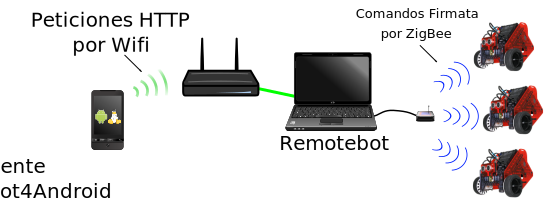
\includegraphics[width=\textwidth]{figures/arquitectura_remotebot}
    \caption{Esquema de conexión de Remotebot}
    \label{fig:arquitectura_remotebot}
\end{figure}


\section{Alternativas similares a XRemotebot}

Existen diferentes alternativas para controlar robots o microcontroladores
de forma remota, muchas de estas se agrupan bajo la denominación
``Internet of Things'', en este capítulo se describirán algunas de las
más destacadas y las más similares a XRemotebot.

% FIXME: mmmm NO SE SI ESTO DEBERÍA ESTAR EN UN CAPITULO APARTE.....  LO HABLAMOS LUEGO

\subsection{Educabot}
%~\citep{_educabot_2015}[REF]%
El proyecto Educabot~\footnote{\url{http://www.educabot.org/}} tiene por
objetivos enseñar tecnología a niños y adultos a través
del uso, programación y construcción de robots. En el sitio del proyecto
se ofertan cursos orientados a los distintos niveles.

% FIXME: ES ORIGINARIO DE ..... EN ESCUELAS? EN ONGS? DONDE SE LOS USA?

En la parte de construcción este proyecto plantea un modelo de robot denominado
``Rolo'' para los jóvenes de más de 10 años, mientras que para los más chicos
se plantean actividades con el robot ``elBrian'' que incluyen
controlarlo a través de una interfaz Web que muestra las imágenes emitidas
por la cámara incorporada en este robot y además permite controlarlo con
botones en pantalla que determinan en qué dirección debe moverse el robot
(figura~\ref{fig:elbrian}).

\begin{figure}
    \centering
    \includegraphics[width=0.5\textwidth]{figures/elbrian-1}
    \caption{Pantalla principal de elBrian (en el recuadro rojo normalmente
        se muestra la cámara de el robot)}
    \label{fig:elbrian}
\end{figure}

Las tecnologías utilizadas en la interfaz web de ``elBrian'' coinciden en gran
parte con las utilizadas en el desarrollo de XRemotebot, pero el objetivo del
servidor CUAL???? es controlar un único robot en un ambiente local y además este servidor
se instala en el robot cuestión que sería imposible en los robots basados en
microcontroladores AVR y Parallax (ojo!!!!  ESTO NOMBRALO ANTES PLEASE!!! ) a los que XRemotebot se encuentra dirigido.


El servidor web de ``elBrian'' está implementado usando el framework Tornado,
Websockets, mjpg-streamer, opencv y JSON. El mismo está diseñado para ejecutarse
en el robot ya que el mismo está basado en una placa RaspberryPi, la cuál
cuenta con un procesador ARM perfectamente capaz de ejecutar un sistema
operativo completo como GNU/Linux y de soportar el intérprete oficial de Python.

Mientras que este servidor coincide en gran medida en la elección de lenguaje
y bibliotecas utilizadas su implementación es específica para el robot ``elBrian''
y no podría ser portada para robots con menores capacidades de procesamiento
sin una reescritura significativa. Además el protocolo utilizado no contempla
el acceso a valores de sensores, los únicos mensajes que permite enviar
al robot son movimientos.

\begin{itemize}
    \item Educabot \url{http://www.educabot.org/}
    \item Código fuente de ``elBrian'' \url{https://github.com/educabot/elBraian}
\end{itemize}

\subsection{Gobot con cppp-io}

Gobot {REF} es una biblioteca que permite controlar robots programando en el lenguaje
Go[REF], esta biblioteca soporta el protocolo Firmata (IDEM CON ESTAS COSAS.... ACLARA, PONE REFERENCIAS O NOMBRLAS ANETES) para controlar robots
conectados directamente a través de una interfaz serial, como es el caso
de los robots Multiplo N6, y soporta la API cppp-io{REF] que define una API JSON
que permite el acceso a la información y control de robots a través de la Web.

Gobot además tiene compatibilidad con distintos sensores y robots, además de
placas utilizadas normalmente en la construcción de robots como Arduino,
Raspberry Pi, Intel Edison y Beaglebone Black.

Este proyecto es interesante como base para desarrollar algún proyecto
similar a XRemotebot en Go, pero requeriría además la reimplementación
del módulo de Python DuinoBot que controla, a través de una versión
modificada del protocolo Firmata, a los robots Multiplo N6 y por otro
lado los robots Scribbler tampoco aparecen en la lista de robots soportados.

\begin{itemize}
    \item Gobot \url{http://gobot.io}
    \item Especificación de cppp-io \url{https://github.com/hybridgroup/cppp-io/}
\end{itemize}

\subsection{Tele Toyland}

Este sitio provee acceso a varios dispositivos a través de una interfaz web,
por ejemplo es posible controlar un cabezal con una punta que dibuja sobre
una caja de arena, basta con hacer clic sobre las posiciones sobre las cuales
se quiere que pase la punta y presionar el botón ``go'' para que el cabezal
empiece a moverse dibujando lo pedido, en este y el resto de los experimentos
disponibles en el sitio los resultados se pueden ver a través de un streaming
de video.

El sitio no provee detalles del software, ni el protocolo utilizado.

\begin{itemize}
    \item \url{http://www.teletoyland.com}
\end{itemize}

% FIXME
%\subsection{}
%http://www3.uji.es/~pnebot/Files/Articuls/RemoteProgramming.pdf
%Otro
%http://telerobot.mech.uwa.edu.au/Telerobot/instructions.html
\subsection{DIY}
% www.linuxuser.co.uk/tutorials/control-your-raspberry-pi-robot-from-a-web-connected-device
Finalmente en la consigna de ``do it yourself'' existen diversas guías para
programar servidores que permitan controlar robots o microcontroladores
en general, se puede encontrar un caso muy bien explicado en el sitio
de Adafruit~\url{https://learn.adafruit.com/wifi-controlled-mobile-robot/building-the-web-interface},
este es un buen ejercicio de programación, sobre todo para aprender a
programar servidores que provean una API web y clientes que la consuman. Sin
embargo estas guías son introductorias y el objetivo es crear un servidor
muy simple, similar a lo que fue el servidor Remotebot, pensados para ser
usados en un ambiente local ya que no proveen autenticación en general.


\chapter{Controlando dispositivos de forma remota}\label{cha:arte}

Existen diferentes alternativas para controlar robots o microcontroladores
de forma remota. Muchas de estas se agrupan bajo la denominación
``Internet of Things''\footnote{\url{https://www.iotwf.com/resources/1}}.
En este capítulo se describirán algunas de las
más destacadas entre las más similares a los requerimientos planteados en
esta propuesta.


\section{Educabot}
El proyecto Educabot\footnote{\url{http://www.educabot.org/}} tiene por
objetivo enseñar tecnología a niños y adultos a través
del uso, programación y construcción de robots. En el sitio del proyecto
se ofertan cursos orientados a los distintos niveles y 
en la última conferencia de Python de Argentina (Pyconar 2014) uno de
los cofundadores del proyecto mencionó que se llevan adelante actividades
con los robots
en distintas escuelas de la Ciudad Autónoma de Buenos
Aires\footnote{\url{https://youtu.be/1oCOAtX9OS4}}.

% FIXME: ES ORIGINARIO DE ..... EN ESCUELAS? EN ONGS? DONDE SE LOS USA?
% Son cursos privados según dijo el tipo, pero no tengo de donde citar
% eso no dice nada el sitio.
% FIXME: En el sitio no mencionan nada de los cursos en escuelas lo único
% que encontré es lo de youtube que es una charla en la Pycon del fundador

En la parte de construcción, este proyecto plantea un modelo de robot
denominado
``Rolo'' para los jóvenes de más de 10 años, mientras que para los más chicos
se plantean actividades con el robot ``elBrian'' que incluyen
controlarlo a través de una interfaz web que muestra las imágenes emitidas
por la cámara incorporada en este robot y además permite controlarlo con
botones en pantalla que determinan en qué dirección debe moverse el robot
(figura~\ref{fig:elbrian}).

\begin{figure}
    \centering
    \includegraphics[width=0.5\textwidth]{figures/elbrian-1}
    \caption{Pantalla principal de elBrian (en el recuadro rojo normalmente
        se muestra la cámara de el robot)}
    \label{fig:elbrian}
\end{figure}

Las tecnologías utilizadas en la interfaz web de ``elBrian'' coinciden en gran
parte con las utilizadas en el desarrollo de XRemoteBot, pero el objetivo del
servidor de ``elBrian'' es controlar un único robot en un ambiente local.
Además este servidor
se instala en el robot utilizado,  cuestión que sería imposible en los
robots basados en
microcontroladores AVR y PIC (``Basic Stamp 2`` de Parallax)
a los que XRemoteBot se encuentra dirigido.

%FIXME: fijate de poner aunque sea notas al pie con las referencias de los paquetes o protocolos que nmbras... el que no sabe.. se muere...

El servidor web de ``elBrian'' está implementado usando el framework
Tornado\footnote{\url{http://www.tornadoweb.org/}},
WebSockets\footnote{\url{http://www.websocket.org/}},
mjpg-streamer\footnote{\url{https://github.com/jacksonliam/mjpg-streamer}},
opencv\footnote{\url{http://opencv.org/}}
y JSON\footnote{\url{http://json.org/}}.
El mismo está diseñado para ejecutarse
en el robot ya que el mismo está basado en una placa RaspberryPi, la cuál
cuenta con un procesador ARM perfectamente capaz de ejecutar un sistema
operativo completo como GNU/Linux y de soportar el intérprete oficial de Python.

Mientras que este servidor coincide en gran medida en la elección de lenguaje
y bibliotecas utilizadas, su implementación es específica para el robot ``elBrian''
y no puede ser portada a robots con menores capacidades de procesamiento
sin una reescritura significativa. Además el protocolo utilizado no contempla
el acceso a valores de sensores siendo los únicos mensajes que permite enviar
al robot los comandos de movimientos.

Referencias del proyecto:
\begin{itemize}
    \item Página del proyecto: \url{http://www.educabot.org/}
    \item Código fuente de ``elBrian'': \url{https://github.com/educabot/elBraian}
\end{itemize}

\section{Gobot con cppp-io}

Gobot\footnote{\url{http://gobot.io}}
es una biblioteca que permite controlar robots programando en el lenguaje
Go\footnote{\url{https://golang.org/}}. Esta biblioteca soporta el
protocolo Firmata
para controlar robots
conectados directamente a través de una interfaz serial, como es el caso
de los robots Multiplo N6, y soporta la API
cppp-io\footnote{\url{https://github.com/hybridgroup/cppp-io/}}
que define una API JSON
que permite el acceso a la información y control de robots a través de la Web.

Gobot además tiene compatibilidad con distintos sensores y robots, además de
ser compatible con
placas utilizadas normalmente en la construcción de robots como Arduino,
Raspberry Pi, Intel Edison y Beaglebone Black%
\footnote{\url{http://gobot.io/\#platforms}}.

Este proyecto es interesante como base para desarrollar algún proyecto
similar a XRemoteBot en Go, pero requiere además la reimplementación
del módulo de Python DuinoBot que controla, a través de una versión
modificada del protocolo Firmata, a los robots Multiplo N6. Por otro
lado, los robots Scribbler tampoco aparecen en la lista de robots soportados.

Referencias del proyecto:
\begin{itemize}
    \item Página del proyecto: \url{http://gobot.io}.
    \item Protocolo de su API Web: \url{https://github.com/hybridgroup/cppp-io/}.
\end{itemize}


\section{Cylon.js}

Cylon.js es un proyecto hermano de Gobot y soporta la misma variedad
de dispositivos y también provee una API cppp-io, con la diferencia
de que la biblioteca provista está escrita en Javascript para NodeJS.

Una característica interesante de Cylon.js es que soporta distintos
protocolos para su API remota como ser HTTP, socket.io y la capacidad
de agregar nuevos protocolos con
plugins

\begin{lstlisting}[caption={Cylon.js controlando 2 robots ``sphero'' usando HTTP},
label={lst:cylonjs_ejemplo}]
"use strict";

var Cylon = require("cylon");

// ensure you install the API plugin first:
// $ npm install cylon-api-http
Cylon.api({
  host: "0.0.0.0",
  port: "8080"
});

var bots = {
  "Thelma": "/dev/rfcomm0",
  "Louise": "/dev/rfcomm1"
};

Object.keys(bots).forEach(function(name) {
  var port = bots[name];

  Cylon.robot({
    name: name,

    connections: {
      sphero: { adaptor: "sphero", port: port }
    },

    devices: {
      sphero: { driver: "sphero" }
    },

    work: function(my) {
      every((1).seconds(), function() {
        console.log(my.name);
        my.sphero.setRandomColor();
        my.sphero.roll(60, Math.floor(Math.random() * 360));
      });
    }
  });
});

Cylon.start();
\end{lstlisting}

En el código~\ref{lst:cylonjs_ejemplo} se puede ver un ejemplo de
Cylon.js del lado del servidor exponiendo dos robots de tipo
\textit{sphero} a través de la API HTTP,
una vez ejecutado este código en el servidor, a través de la API se
les podrá enviar un mensaje a los robots
robots que hará que cambien
de color
y se desplacen
rodando\footnote{Los robots sphero son pequeñas esferas \url{http://www.gosphero.com/}.}.

Si bien en la documentación del proyecto se detalla como habilitar
un sistema de login para acceder a la API de forma remota, el mismo
no parece estar diseñado para el acceso concurrente de distintos usuarios
ya que de la documentación no surge que Cylon.js soporte un sistema
de reserva de robots o de exclusión mutua en el acceso a los mismos.

Referencias del proyecto:
\begin{itemize}
    \item Página del proyecto: \url{http://cylonjs.com/}.
\end{itemize}


\section{VCar}

\begin{figure}
    \centering
    \includegraphics[width=0.5\linewidth]{figures/vcar}
    \caption{Interfaz de VCar}
    \label{fig:vcar}
\end{figure}

VCar es un auto a control remoto, cuyo control fue modificado para
se manipulado por software desde  una computadora con GNU/Linux la
cuál permite controlar el robot de forma remota y verlo
a través de una cámara de
video\footnote{\url{http://www.hellspark.com/new/css/vcar/vcar.html}}
(figura~\ref{fig:vcar}).
El acceso al robot es público
aparentemente sin ningún tipo de restricción y la página
si bien no tiene detalles de todo el hardware y el software utilizados
provee algunas fotos de la construcción del
sistema\footnote{\url{http://www.hellspark.com/dm/gallery2/v/projects/robotics/vcar/}}

Referencias del proyecto:
\begin{itemize}
    \item Página del proyecto: \url{http://www.hellspark.com/new/css/vcar/vcar.html}.
    \item Galería de fotos: \url{http://www.hellspark.com/dm/gallery2/v/projects/robotics/vcar/}}
\end{itemize}


\section{Tele Toyland}

Tele Toyland\footnote{\url{http://www.teletoyland.com}} es un sitio que provee acceso a varios dispositivos a través de una interfaz
web. Por ejemplo, es posible controlar un cabezal con una punta que dibuja sobre
una caja de arena. Basta con hacer clic sobre las posiciones sobre las cuales
se quiere que pase la punta y presionar el botón ``go'' para que el cabezal
empiece a moverse dibujando lo pedido. En éste y el resto de los experimentos
disponibles en el sitio, los resultados se pueden ver a través de un streaming
de video.

Entre los proyectos con los que permite interactuar Tele Toyland
se encuentran  2 areneros como el descripto
anteriormente, una torre de leds, una marioneta y laberintos.

El sitio no provee detalles del software, ni el protocolo utilizado. Desde
lo funcional
provee una especie de control remoto para los distintos dispositivos a los
que permite
manipular, en donde se puede, incluso, configurar una serie de instrucciones a ejecutar
en secuencia. Sin embargo no provee una biblioteca que permita controlar
los dispositivos desde un lenguaje de programación.

Referencias del proyecto:
\begin{itemize}
    \item Página del proyecto: \url{http://www.teletoyland.com}.
\end{itemize}
% FIXME
%\section{}
%http://www3.uji.es/~pnebot/Files/Articuls/RemoteProgramming.pdf
%Otro
%http://telerobot.mech.uwa.edu.au/Telerobot/instructions.html
\section{Otros proyectos}
% www.linuxuser.co.uk/tutorials/control-your-raspberry-pi-robot-from-a-web-connected-device



%FIX ME ESTO QUEDA MUY DESCOLGADO..... yo pondŕia algo como 
%Bajo la consigna DIY, o ``do it yourself'' y acá poner un par de ref!!!, existen diversas.....y seguir...., 

Existieron otros sistemas similares en el pasado, pero actualmente se
encuentran fuera de línea por problemas técnicos o bien porque el
experimento terminó como por ejemplo
``TU Freiberg Robotics''\footnote{\url{www.informatik.tu-freiberg.de/\~frobots/}}
que permitía controlar robots en una mini cancha de fútbol,
``WebTruck''\footnote{\url{http://www.webtruck.org/cinteraction_html}} que
permitía controlar distintos vehículos.

También existen otros proyectos que requieren instalar software extra
como ``The UWA Telerobot'' que requiere instalar software propietario
y crear una cuenta para ser utilizado, este proyecto permite controlar
un brazo robótico en un taller.

Finalmente en la consigna de ``do it yourself'' existen diversas guías para
programar servidores que permitan controlar robots o microcontroladores
en general, se puede encontrar un caso muy bien explicado en el sitio
de Adafruit~\url{https://learn.adafruit.com/wifi-controlled-mobile-robot/building-the-web-interface},
este es un buen ejercicio de programación, sobre todo para aprender a
programar servidores que provean una API web y clientes que la consuman. Sin
embargo estas guías son introductorias y el objetivo es crear un servidor
muy simple, similar a lo que fue el servidor RemoteBot, pensados para ser
usados en un ambiente local ya que no proveen autenticación en general.

\section{Conclusiones del capítulo}

Si bien existen proyectos parecidos que brindan al público la posibilidad
de controlar un robot de manera remota, ninguno de estos es una solución
completa al problema de enseñar a programar usando
robots de forma remota y permitiendo a distintos usuarios reservar
temporalmente distintos
robots de forma que no haya conflicto en la interacción entre los usuarios.

%El capítulo 3 describe el protocolo de capa de aplicación diseñado para
%este servidor y las modalidades de operación del servidor.
\chapter{Protocolo de capa de aplicación}\label{ch3}

Como se describió anteriormente XRemoteBot utiliza el protocolo WebSocket como
protocolo de la capa de transporte y mensajes codificados con JSON como
protocolo de la capa de aplicación, el propósito de este capítulo es describir
este protocolo de capa de aplicación y detallar los motivos por los cuales
se modeló el protocolo de esta manera.


El protocolo fue diseñado pensando que el mismo debería representar los
distintos comandos envíados a los robots como si fueran mensajes a objetos
del paradigma de programación orientado a objetos
este diseño por un lado mapea de forma muy directa los mensajes de la API
con los métodos que un programador utilizaría para controlar a los robots
usando la biblioteca DuinoBot y por otro lado provee un alto grado de
flexibilidad a la hora de agregar nuevos tipos de mensajes a la API sin
necesidad de reescribir grandes porciones de código.

En algunos de los lenguajes orientados a objetos más populares como Python
o Ruby al ejecutar un método pueden ocurrir básicamente dos cosas:
se puede obtener un valor de resultado o bien un error
en tiempo de ejecución en la forma de una excepción. Para modelar este
comportamiento el servidor XRemoteBot cuenta con dos tipos de mensajes
de respuesta:
``value'' que retorna el valor resultante de ejecutar el método invocado y
``error'' que representa un error que típicamente se representaría como
una excepción, los mensajes de error de XRemoteBot tienen como contenido
un mensaje que describe el error, los clientes pueden tomar este mensaje
de error y mostrarlos en pantalla o usarlos como descripción de una
excepción como se hace en el cliente Python por ejemplo.

Tanto para los parámetros, como para los valores de respuesta, los tipos
de datos representables de forma nativa con JSON resultan suficientes para
implementar una API similar a la de DuinoBot. Internamente XRemoteBot
convierte los valores, objetos y arrays de JSON a distintos tipos de
datos de Python de la forma descripta en la
tabla~\ref{tbl:rel_json_python}, siguiendo en general las transformaciones
realizadas por defecto por las funciones de procesamiento de el módulo
JSON de la biblioteca estándar d
Python~\footnote{\url{https://docs.python.org/3/library/json.html}}
excepto en algunos mensajes donde los valores de
tipo \texttt{number} de JSON se convierten explícitamente (en realidad
se utilizan funciones provistas por Tornado para hacer la conversión
de JSON a objetos y de objetos a JSON, pero estas funciones utilizan
a su vez el módulo JSON de
Python)~\footnote{\url{http://tornado.readthedocs.org/en/latest/escape.html\#tornado.escape.json_encode}}.

\begin{table}
    \centering
    \begin{tabu}{l|l}
        JSON & Python \\
        \hline
        \texttt{string} & \texttt{str} \\
        \texttt{number} & \texttt{int} o \texttt{float}~\footnote{Dependiendo
        del mensaje invocado
        puede ser interpretado como \texttt{int} o \texttt{float}.}\\
        \texttt{object} & \texttt{dict} \\
        \texttt{array}  & \texttt{list} \\
        \texttt{true}/\texttt{false} & \texttt{True}/\texttt{False} (bool) \\
        \texttt{null} & \texttt{None} \\
    \end{tabu}
    \caption{Relación entre los tipos y constantes de JSON y los usados en
    Python}
    \label{tbl:rel_json_python}
\end{table}

\section{Mensajes del cliente al servidor}

Los mensajes al servidor son objetos JSON con dos campos obligatorios y dos
opcionales, estos campos son:

\begin{description}
    \item[\texttt{entity}] su valor es un string que describe conceptualmente
        el receptor del mensaje (obligatorio).
    \item[\texttt{method}] su valor es un string con el nombre del método a
        invocar (obligatorio).
    \item[\texttt{args}] su valor es un array posiblemente vacío con los
        argumentos que deben pasarse al método invocado (opcional).
    \item[\texttt{msg\_id}] si está presente el servidor incorpora este
        campo con su valor original en la respuesta, sirve para identificar a
        qué petición
        corresponde cada respuesta en implementaciones asincrónicas
        como la de Javascript.
\end{description}

En la actual implementación los valores posibles de \texttt{entity} son
\texttt{``global''} y \texttt{``robot''}, el primero
representa acciones globales como el login y el último representa una
abstracción de los robots soportados por XRemoteBot.

La entidad ``global'' soporta los métodos:
\begin{description}
    \item[\texttt{authentication\_required}] no recibe argumentos, retorna
        \texttt{true} si el servidor está configurado para requerir
        autenticación y \texttt{false} en caso contrario.
    \item[\texttt{authenticate}] recibe un string, si el string se corresponde
        con la \texttt{api\_key} de algún usuario y esa \texttt{api\_key} no
        ha expirado retorna \texttt{true} y \texttt{false} en caso contrario.
\end{description}

Entre otros la entidad ``robot'' soporta los métodos:
\begin{description}
    \item[\texttt{backward}] recibe un objeto que identifica a un robot
        específico, una velocidad y un tiempo en segundos,
        mueve el robot hacia atrás el tiempo indicado y luego contesta
        al cliente. Si no se envía el parámetro de tiempo el robot se mueve
        de forma indefinida.
    \item[\texttt{forward}] ídem moviendo el robot hacia adelante.
    \item[\texttt{turnLeft}] ídem girando a izquierda.
    \item[\texttt{turnRight}] ídem girando a derecha.
    \item[\texttt{getObstacle}] recibe un objeto que identifica a un robot,
        opcionalmente una distancia y retorna
        \texttt{true} si hay un obstáculo a una distancia menor o igual a la
        indicada, si no se envía la distancia se asume un valor por defecto.
    \item[\texttt{getLine}] recibe un objeto que identifica a un robot y
        retorna un \texttt{array}
        con los valores de los sensores de línea del robot.
\end{description}

Opcionalmente un modelo dado de robot puede soportar otros métodos o retornar
error en alguno de los métodos anteriores.

La posiblidad que tienen los métodos con tiempo como \texttt{backward} de
contestar la petición varios segundos después de recibirla sin afectar
el funcionamiento del servidor ni demorar innesesariamente al resto de los
clientes está dada por el soporte de asincronismo del framework Tornado.

\section{Mensajes del servidor a los clientes}

El servidor responde a los clientes con mensajes que contienen una
entrada \texttt{response}, esta entrada identifica el tipo de respuesta
que puede ser \texttt{value} o \texttt{error}, si el cliente envío un
campo \texttt{msg\_id} en la petición el servidor incorporará además
un campo \texttt{msg\_id} idéntico en la respuesta correspondiente
a esa petición (como se mencionó anteriormente para soportar
clientes asincrónicos de forma correcta).

Campos de los mensajes \texttt{value}:
\begin{description}
    \item[\texttt{response}] el string \texttt{``value''}.
    \item[\texttt{value}] el valor retornado por el método (puede ser
        cualquier valor soportado por JSON).
    \item[\texttt{msg\_id}] si la petición tenía \texttt{msg\_id} se
        copia el mismo, sino este campo se omite.
\end{description}

Campos de los mensajes \texttt{error}:
\begin{description}
    \item[\texttt{response}] el string \texttt{``error''}.
    \item[\texttt{message}] un mensaje de error descriptivo.
    \item[\texttt{msg\_id}] si la petición tenía \texttt{msg\_id} se
        copia el mismo, sino este campo se omite.
\end{description}

Los mensajes \texttt{value} representan los valores de respuesta de
los métodos invocados, para los mensajes que requieren
un tiempo de demora el servidor contestará con el mensaje \texttt{value}
una vez transcurrido ese tiempo, para no demorar la atención de peticiones
de otros clientes el servidor utiliza las funcionalidades provistas por
Tornado para atender peticiones de forma asíncrona~\citep{dory_2012}. Por
otro lado los mensajes \texttt{error} representan eventos anómalos que
generalmente en un sistema no distribuido se modelarían utilizando
excepciones, por ejemplo errores de codificación, peticiones a recursos
ocupados, etc...

\section{Ejemplos de interacción entre los clientes y el servidor}

Al comenzar la conexión entre el cliente y el servidor, se intercambian
los primeros mensajes donde el cliente pregunta al servidor si el
mismo requiere autenticación y si es así envía la \textit{API key}
correspondiente. En la tabla~\ref{tbl:ej_autenticacion} se detalla
el intercambio de mensajes entre un cliente y el servidor en un
caso de autenticación exitoso con un cliente que envía un \texttt{msg\_id},
como se puede ver el \texttt{msg\_id}
no tiene por qué ser consecutivo con el del mensaje anterior, incluso
puede llegar a ser un string, las únicas restricciones sobre el
\texttt{msg\_id} son que tiene que ser copiado por el servidor
en las respuestas y que el valor debe poder ser utilizado como
identificador de un atributo (usando notación con corchetes) en un
objeto Javascript, es decir puede ser un número o un string
arbitrario~\footnote{\url{https://developer.mozilla.org/en-US/docs/Web/JavaScript/Reference/Operators/Property\_Accessors}}.

\begin{table}
    \centering
    \begin{tabular}{|m{.49\textwidth}|m{.49\textwidth}|}
        \hline
        \textit{Petición del cliente} & \textit{Respuesta del servidor} \\
        \hline
\begin{Verbatim}[fontsize=\footnotesize]
{
    "entity": "global",
    "method": "authentication_required",
    "msg_id": 0
}
\end{Verbatim}
&
\begin{Verbatim}[fontsize=\footnotesize]
{
    "response": "value",
    "value": true,
    "msg_id": 0
}
\end{Verbatim}
\\
\hline
\begin{Verbatim}[fontsize=\footnotesize]
{
    "entity": "global",
    "method": "authenticate",
    "args": ["16758efc752c1d97381e6"],
    "msg_id": 20
}
\end{Verbatim}
&
\begin{Verbatim}[fontsize=\footnotesize]
{
    "response": "value",
    "value": true,
    "msg_id": 20
}
\end{Verbatim}
\\
\hline
    \end{tabular}
    \caption{Ejemplo de secuencia de autenticación}
    \label{tbl:ej_autenticacion}
\end{table}

Otra secuencia de operaciones típica para XRemoteBot es mover un robot
y luego pedir los valores de alguno de sus sensores, en la
tabla~\ref{tbl:ej_movimiento_y_sensor} se puede ver un caso donde se
mueve el robot hacia adelante durante 1 segundo y luego consulta si
existe algún obstáculo a 10 centímetros o menos del robot, en el primer
argumento de los mensajes
envíados a la entidad \textit{robot} se puede ver el objeto que identifica
al robot específico a utilizar.

\begin{table}
    \centering
    \begin{tabular}{|m{.49\textwidth}|m{.49\textwidth}|}
        \hline
        \textit{Petición del cliente} & \textit{Respuesta del servidor} \\
        \hline
\begin{Verbatim}[fontsize=\footnotesize]
{
    "entity": "robot",
    "method": "forward",
    "args": [50, 1],
    "msg_id": 40
}
\end{Verbatim}
&
\begin{Verbatim}[fontsize=\footnotesize]
{
    "response": "value",
    "value": null,
    "msg_id": 40
}
\end{Verbatim}
\\
\hline
\begin{Verbatim}[fontsize=\footnotesize]
{
    "entity": "robot",
    "method": "getObstacle",
    "args": [{model: "n6", id: 4}, 10],
    "msg_id": 42
}
\end{Verbatim}
&
\begin{Verbatim}[fontsize=\footnotesize]
{
    "response": "value",
    "value": false,
    "msg_id": 42
}
\end{Verbatim}
\\
\hline
    \end{tabular}
    \caption{Ejemplo de movimiento y acceso a sensores de un robot}
    \label{tbl:ej_movimiento_y_sensor}
\end{table}

Por último en la tabla~\ref{tbl:ej_error} se puede ver un mensaje de error
típico cuando el cliente envía una petición mal formada donde no existe
el campo \textit{method} obligatorio, notar que este mensaje a diferencia
de los anteriores no tiene un campo \textit{msg\_id} pero esto no causaría
ningún error ya que este campo no es obligatorio, el único error en la
petición es la ausencia de \textit{method}.

\begin{table}
    \centering
    \begin{tabular}{|m{.49\textwidth}|m{.49\textwidth}|}
        \hline
        \textit{Petición del cliente} & \textit{Respuesta del servidor} \\
        \hline
\begin{Verbatim}[fontsize=\footnotesize]
{
    "entity": "robot",
}
\end{Verbatim}
&
\begin{Verbatim}[fontsize=\footnotesize]
{
    "response": "error",
    "message": "\"entity\" and \"method\"
                are mandatory fields"
}
\end{Verbatim}
\\
\hline
    \end{tabular}
    \caption{Ejemplo de un mensaje de error ante una petición mal formada}
    \label{tbl:ej_error}
\end{table}

\section{Modalidades del servidor}

A fin de hacer que el servidor pueda exponerse al público se cuenta con
un sistema con autenticación por \textit{API key}, pero estas claves
son largas resultando díficil recordarlas y escribirlas sin errores. En
ámbitos locales como puede ser una red wifi en un aula este mecanismo
de autenticación puede resultar molesto e innecesario, por lo que el
servidor es configurable de forma tal que se puede deshabilitar este
sistema de autenticación. Para que el servidor opere sin requerir
una \textit{API key} a los clientes basta con configurar la opción
\texttt{public\_server} en \texttt{False} dentro del archivo
\textit{configuration.py}.



% El capítulo 4 describe la implementación de los clientes y el modo de uso
% de cada uno destacando algunas diferencias y decisiones de diseño en la
% implementación en Javascript.

\chapter{Implementación de los clientes}\label{ch4}
Los clientes hosted no tienen video % FIXME
Cuestiones de estilo casing copiando duinobot

Se implementaron 3 clientes para permitir el uso de XRemoteBot desde 3
lenguajes de programación distintos: Python, Ruby y Javascript. Este último
en el navegador.

\section{Cliente Python}\label{ch4:python}
El uso del cliente Python es muy similar al uso directo de los robots con la
biblioteca DuinoBot aunque la implementación es bastante diferente por el protocolo
subyacente.

El cliente Python utiliza un solo módulo que no pertenece a la biblioteca estándar
de Python, el módulo para acceso a WebSockets
\textit{websocket-client}~\footnote{\url{https://pypi.python.org/pypi/websocket-client}}
que cuenta, además de con una interfaz asincrónica, con una interfaz de ``bajo nivel''
sincrónica similar a la interfaz tradicional de Sockets.

\begin{lstlisting}[language=Python,
caption={Ejemplo con XRemoteBot para Python},label=lst:ejemplo_xremotebot_python]
from xremotebot import *
server = Server('ws://xremotebot.example:8000/api', 'api_key')
robot = server.fetch_robot()
robot.forward(100, 1)
robot.backward(50, 2)
print(robot.getObstacle())
\end{lstlisting}


Las operaciones con demoras, como los movimientos se implementan localmente
utilizando 2 mensajes y la función \texttt{time.wait()} de Python. De esta
forma
invocar al método \texttt{robot.forward(100, 1)} se traduce en los mensajes
de
la figura~\ref{fig:mensajes_xremotebot_python_json}. Como todos los métodos
de movimiento
proveen esta funcionalidad de demora, la misma implementada en el
\textit{decorator}~\footnote{Esto es un decorator de Python, no confundir
con el patrón de diseño. \url{https://www.python.org/dev/peps/pep-0318/}}
\texttt{xremotebot.timed} a fin de evitar repetición de código.

\begin{lstlisting}[language=Python,
caption={Mensajes generados al invocar \texttt{robot.forward(100, 1)} en
XRemoteBot para Python}, label=lst:ejemplo_xremotebot_python_json]
{
    "entity": "robot",
    "method": "forward",
    "args": [100]
}
# Después de 1 segundo...
{
    "entity": "robot",
    "method": "stop",
    "args": []
}
\end{lstlisting}


\section{Cliente Ruby}\label{ch4:ruby}

Las gemas que proveen soporte para WebSockets en Ruby proveen una API
asincrónica que no es deseable para este proyecto por lo que me incliné
por incorporar el código del
proyecto~\footnote{\url{https://github.com/gimite/web-socket-ruby}}
al cliente Ruby de XRemoteBot, este proyecto no se encuentra empaquetado
en forma de gema pero provee una API sincrónica que permite implementar
el cliente Ruby de XRemoteBot para que se comporte de una forma muy similar
a la biblioteca DuinoBot original.

\begin{lstlisting}[language=Ruby,
caption={Ejemplo usando XRemoteBot para Ruby},
label=lst:ejemplo_xremotebot_ruby]
require 'xremotebot'
server = XRemoteBot::Server.new('ws://xremotebot.example:8000/api',
                                'api_key')
robot = server.fetch_robot
robot.forward 100, 1
robot.backward 50, 2
print robot.getObstacle
\end{lstlisting}



\section{Cliente Javascript}\label{ch4:javascript}

\subsection{API Javascript y asincronismo}
Como se mencionó con anterioridad, gran parte de las decisiones de diseño de XRemoteBot
se hicieron para permitir la implementación de un cliente Javascript, pero dado el hecho
de que Javascript dentro del entorno de un navegador Web se comporta de forma asincrónica
no fue posible implementar un cliente Javascript cuyo uso se asemeje al de la biblioteca
de Python DuinoBot.

Para ilustrar esta problemática se puede tomar en consideración el 
código~\ref{lst:ejemplo_duinobot}
típico hecho usando DuinoBot en Python y analizar los inconvenientes para replicar
algo similar en Javascript.

\begin{lstlisting}[language=Python,
caption={Ejemplo típico usando DuinoBot},label=lst:ejemplo_duinobot]
from duinobot import *
board = Board()
robot = Robot(board, 10)
robot.forward(100, 1)
robot.backward(50, 2)
print(robot.getObstacle())
\end{lstlisting}


Las líneas 2 y 3 del ejemplo de la código~\ref{lst:ejemplo_duinobot} son
operaciones que retornan objetos, en XRemoteBot la línea 2 no tiene sentido
ya que la placa a la que está conectado el robot está predefinida en el
servidor, pero la línea 3 sí es necesaria para obtener una instancia de un
robot no reservado, estas operaciones que retornan un valor el XRemoteBot
se dividen en un mensaje de petición y uno de respuesta, el problema
es que por el asincronismo de Javascript y de la API de WebSockets no
es posible determinar en que momento llegará la respuesta con el valor
retornado y la única forma de bloquear la ejecución del script hasta que
llegue la respuesta sería hacer ``busy waiting'', lo cuál puede llegar a
bloquear la pestaña del navegador ya que los navegadores típicamente usan
un solo thread compartido entre el renderizado de la página, manejo de
eventos y ejecución del código Javascript asociado a la página.

En tanto las líneas 4 y 5 si bien no retornan un valor deben ejecutarse
en orden, y la línea 5 en este caso debe ejecutarse precisamente 1 segundo
después de la ejecución de la línea 4, también la línea 6 deberá ejecutarse
2 segundos después de la línea 5 ya que no es lo mismo preguntar si hay
un obstáculo cuando el robot aún no retrocedió, esto que parece muy obvio
y natural en la mayoría de los lenguajes de programación no es posible
en Javascript (dentro del navegador, con intérpretes como NodeJS sí es
posible) y el orden de ejecución y demora no se puede lograr simplemente
poniendo una instrucción debajo de otra.\footnote{FIXME}


La solución encontrada a este problema fue el uso de
\textit{Promises}~\citep{ECMA-262},
las \textit{Promises} proveen un mecanismo para ejecutar instrucciones,
que dependen de los resultados o de la terminación de eventos asincrónicos,
las \textit{Promises} permiten tener secuencia e interdependencia entre los
mensajes enviados a los
robots.
Si bien el objeto \textit{Promise} está en proceso de estandarización,
los navegadores Google Chrome, Firefox, Internet Explorer, Opera y Safari las
soportan~\footnote{\url{https://developer.mozilla.org/en-US/docs/Web/JavaScript/Reference/Global_Objects/Promise}}.
El problema de esta solución es que la sintaxis de un script XRemoteBot en
Javascript usando \textit{Promises}
resulta bastante distinta de la sintaxis de un script DuinoBot como resulta
evidente
en el código~\ref{lst:ejemplo_xremotebot_javascript} donde se muestra un
script equivalente
al del código~\ref{lst:ejemplo_duinobot} escrito en Javascript.

\begin{lstlisting}[language=C,
caption={Ejemplo de XRemoteBot en Javascript},
label=lst:ejemplo_xremotebot_javascript]
var server = new Server('xremotebot.example:8000', 'api-key');
server.onConnect(function(){
    server.fetch_robot().then(function(robot){
        robot.forward(100, 1).then(function(){
            robot.backward(50, 2).then(function(){
                robot.getObstacle().then(function(obstacle){
                    println(obstacle);
                })
            })
        })
    });
});
\end{lstlisting}

Como se puede ver después de cada acción bloqueante, es decir cada método que
provoque una demora, y de cada método que retorne un valor útil, como
\texttt{Robot\#getObstacle()}, se invoca el método \texttt{Promise\#then()} con
una función anónima como argumento. Esta función que se pasa por argumento al
then se ejecutará si la \textit{Promise} se ``resuelve'', en el caso de
XRemoteBot la \textit{Promise} se ``resuelve'' cuando el servidor
responde al mensaje que generó la \textit{Promise}.
Este mecanismo se logró identificando cada mensaje con un \texttt{msg\_id},
manteniendo un objeto Javascript (usado como si fuera un \texttt{dict}
o \texttt{HashMap}) con el identificador como clave y la promesa
correspondiente a cada uno los mensajes cuyas respuestas están pendientes
como valor. Dentro del callback \texttt{onmessage} del WebSocket utilizado
al recibir una respuesta se busca el \texttt{msg\_id} en el objeto de
mensajes con respuesta pendiente y se ``resuelve'' la promesa correspondiente
a este mensaje. De esta manera se ejecuta la siguiente función (pasada como
argumento a \texttt{Promise\#then}) siguiendo con el flujo del programa
en orden y con la demora necesaria. En el
código~\ref{lst:ejemplo_xremotebot_javascript_promises} se muestra esta primer
implementación.


\begin{lstlisting}[language=C,
caption={Ejemplo simplificado de la implementación de XRemoteBot con
Promises dentro del constructor Server en remotebot.js},
label=lst:ejemplo_xremotebot_javascript_promises]
this.send_ws_msg = function(msg){
    var promise;
    promise = new Promise(function(resolve, reject){
        that.pending_msgs[msg_id] = {resolve: resolve, reject: reject};
    });
    msg['msg_id'] = msg_id;
    that.ws.send(JSON.stringify(msg));
    return promise;
}
// ...
this.ws.onmessage = function(msg){
    msg = JSON.parse(msg.data);
    if (msg['msg_id'] !== undefined){
        var executor = that.pending_msgs[msg['msg_id']];
        delete that.pending_msgs[msg['msg_id']];
        executor.resolve(msg);
    }
};
\end{lstlisting}


Evidentemente esta forma de programar resulta engorrosa y poco práctica,
por lo que se añadieron
lógica y estructuras de datos extra que serializan en envío de mensajes al
servidor, enviando de a un mensaje por vez (el objeto Javascript con
mensajes con respuesta pendiente tendrá a lo sumo una entrada)
y encolando los mensajes sobrantes
en una cola de mensajes demorados (\texttt{Server\#delayed}), cuando
el servidor contesta el mensaje enviado anteriormente se toma un mensaje
de la cola si lo hubiere y se lo envía al servidor. De esta manera
se garantiza la demora necesaria entre la ejecución de cada método
del robot, sin embargo para obtener los valores de retorno de los métodos,
como en el caso de los métodos de acceso a los sensores, sigue siendo
necesario el uso del método \texttt{Promise\#then}. A pesar de esto último
como se puede ver en el código~\ref{lst:ejemplo_xremotebot_javascript_cola}
con estas modificaciones es posible hacer que el cliente Javascript
tenga una API más limpia y usable, esta última versión es la definitiva
para este trabajo.

\begin{lstlisting}[language=C,
caption={Ejemplo de XRemoteBot en Javascript con empleo de una cola para
serializar mensajes},
label=lst:ejemplo_xremotebot_javascript_cola]
var server = new Server('xremotebot.example:8000', 'api-key');
server.fetch_robot().then(function(robot){
    robot.forward(100, 1);
    robot.backward(50, 2);
    robot.getObstacle().then(function(obstacle){
        println(obstacle);
    });
});
\end{lstlisting}


Una solución alternativa para lograr imitar tanto como sea posible la
API de DuinoBot puede ser utilizar un intérprete Javascript implementado en
Javascript como
JS-Interpreter~\footnote{\url{https://github.com/NeilFraser/JS-Interpreter}},
pero requeriría modificar el intérprete para lograr una ejecución paso a paso
controlada por el flujo de mensajes a través de la conexión con WebSockets,
además de agregar complejidad, este tipo de intérpretes no accede a un entorno
compreto como lo hace el intérprete incorporado en los navegadores y puede
tener incompatibilidades o funcionalidades no implementadas, en este caso
por ejemplo JS-Interpreter no soporta interrupciones y no puede interactuar
directamente con DOM, otra opción es
Hypnotic~\footnote{\url{http://coolwanglu.github.io/hypnotic/web/demo.html}}
que utiliza el intérprete Narcissus y provee una función \texttt{sleep()} que
demora la ejecución del código como se desea para este proyecto, pero el
invoveniente de Hypnotic es que por el momento solamente funciona en el
navegador
Firefox~\footnote{\url{https://github.com/coolwanglu/hypnotic/wiki\#limitations}}.


\subsection{Interacción con DOM y JQuery}

\subsection{Interfaz Web y streaming de video}

La interfaz Web de XRemoteBot, que está pensada principalmente para los casos
de uso donde los clientes están en una ubicación geografica distinta a la de
los robots provee login, acceso a la visualización y renovación de una
clave alfanumérica única por cada usuario denominada \textit{API key} que
permite reservar y controlar los robots sin la necesidad de exponer el nombre
de usuario y contraseña, y una página que permite ver los robots en vivo por
video opcionalmente controlandolos con un script Javascript.

Login y renovación de API, doc

La interfaz web pensada para ser utilizada en conjunto con el cliente
Javascript (aunque puede ser accedida sin problemas aún si se usa
otro de los clientes) provee un area de texto para escribir el script
a ejecutar % FIXME
para la misma se utilizó CodeMirror ...

Un area de texto que simula la salida de una terminal, en la misma
se pueden ver mensajes de log generados con la función
\texttt{rblog} que pueden ser habilitados o deshabilitados desde un
checkbox y mensajes impresos con la función \texttt{rbprintln}.

Un area de video destinada a emisiones en vivo que muestren la posición
del robot, el mismo no requiere ningún plugin ya que se utilizó
\texttt{jsmpeg}~\footnote{\url{https://github.com/phoboslab/jsmpeg}}
que permite emitir video en vivo usando WebSockets y renderizarlo
en el navegador en un elemento Canvas, de esta manera se logró tener
video en vivo utilizando características estándar de HTML5.

\chapter{Clientes de XRemoteBot}\label{cha:clientes}

La implementación de XRemoteBot para esta tesina incluye tres clientes en distintos
lenguajes de programación: Python, Ruby y Javascript. Este último diseñado para ejecutarse
en el entorno de un navegador web.

Estos clientes tienen distintas características y principalmente el que más
difiere de los demás es el cliente Javascript ya que es una implementación a
ser ejecutada en un navegador web con las restricciones que esto trae, pero
con la ventaja de que
se encuentra integrado con la vista web de XRemoteBot por lo que cuenta con una
vista de la cámara que integra en una misma pantalla la acción de programar del
usuario con el resultado de la ejecución de dicho código.

En general, se intentó mantener el estilo de programación del módulo DuinoBot
original de la forma más fiel posible. En el caso de Javascript por
limitaciones del entorno
no se logró imitar este estilo tan fielmente como en los otros clientes.

\section{Cliente Python}\label{sec:python}
El uso del cliente Python es muy similar al uso directo de los robots con la
biblioteca DuinoBot, aunque la implementación es bastante diferente por el protocolo
subyacente.

El cliente Python utiliza un solo módulo que no pertenece a la biblioteca estándar
de Python: el módulo para acceso a WebSockets
\textit{websocket-client}\footnote{\url{https://pypi.python.org/pypi/websocket-client}}
que cuenta, con una interfaz asincrónica y con una interfaz de ``bajo nivel''
sincrónica similar a la interfaz tradicional de
Sockets\footnote{\url{http://pubs.opengroup.org/onlinepubs/7908799/xns/syssocket.h.html}},
lo que hace más
natural imitar una biblioteca como DuinoBot.

\begin{lstlisting}[language=Python,
caption={Ejemplo con XRemoteBot para Python},label=lst:ejemplo_xremotebot_python]
from xremotebot import *
server = Server('ws://xremotebot.example:8000/api', 'api_key')
robot = Robot(server, server.fetch_robot())
robot.forward(100, 1)
robot.backward(50, 2)
print(robot.getObstacle())
\end{lstlisting}

En el código~\ref{lst:ejemplo_xremotebot_python} se muestra
un script sencillo creado usando el cliente para Python de XRemoteBot. Este
script reserva un robot en la línea 3, luego lo hace avanzar
a velocidad máxima por 1 segundo, lo hace girar a velocidad media
durante 2 segundos y finalmente imprime en pantalla un valor booleano
que indica si existe algún obstáculo enfrente del robot.

Los movimientos, que pueden recibir por parámetro un tiempo de demora,
se implementan en el cliente
utilizando dos mensajes (uno que comienza el movimiento y otro que lo detiene)
y la función \texttt{time.sleep()} de Python,
esta función suspende la ejecución del hilo actual durante el número
de segundos que se envíe como parámetro. De esta
forma
invocar el método \texttt{robot.forward(100, 1)} en el cliente provoca que
el mismo envíe al servidor los mensajes del
código~\ref{lst:ejemplo_xremotebot_python_json} con una pausa de un segundo
entre ellos. Como todos los métodos de movimiento
proveen esta funcionalidad de demora, la misma está implementada en el
\textit{decorator}\footnote{Esto es un decorator de Python, no confundir
con el patrón de diseño. \url{https://www.python.org/dev/peps/pep-0318/}}
\texttt{xremotebot.timed} a fin de evitar la repetición de código.

\begin{lstlisting}[language=Python,
caption={Mensajes generados al invocar \texttt{robot.forward(100, 1)} en
XRemoteBot para Python}, label=lst:ejemplo_xremotebot_python_json]
{
    "entity": "robot",
    "method": "forward",
    "args": [100]
}
# Después de 1 segundo...
{
    "entity": "robot",
    "method": "stop",
    "args": []
}
\end{lstlisting}


\section{Cliente Ruby}\label{ch4:ruby}

Las gemas (en Ruby el formato de habitual de los paquetes de software
se denomina ``gema'' o, en inglés, ``gem''~\citep{thomas_2013})
que proveen soporte para WebSockets en Ruby cuentan con una API
asincrónica que no es adecuada para este proyecto.
Por esto originalmente se analizó incorporar el código del proyecto
\textit{web-socket-ruby}\footnote{\url{https://github.com/gimite/web-socket-ruby}}
al cliente Ruby de XRemoteBot. Este proyecto no ese encuentra empaquetado en
forma de gema, pero provee una API sincrónica que permiría implementar el
cliente Ruby de XRemoteBot
con una interfaz similar a la biblioteca DuinoBot original.
Sin embargo este proyecto no funciona
con servidores modernos de WebSockets. Por ello, en su lugar,
se utilizó la gema \textit{websocket}\footnote{\url{https://github.com/imanel/websocket-ruby}}
que no es una implementación completa
del protocolo, sino que es una biblioteca de bajo nivel que
solamente permite codificar y decodificar mensajes del protocolo, pero no provee
acceso a la red.

Para proveer cierto nivel de abstracción en el acceso a los WebSockets
se implementó la clase
\texttt{WS} que provee la funcionalidad requerida
usando la clase TCPSocket\footnote{\url{http://ruby-doc.org/stdlib-2.1.0/libdoc/socket/rdoc/TCPSocket.html}}
de Ruby para el acceso a la red y
la gema \textit{websocket} para codificar y decodificar los mensajes intercambiados.
Esta implementación se diseñó para que provea una interfaz similar a la de
\textit{websocket-client}\footnote{\url{https://pypi.python.org/pypi/websocket-client}}.

La implementación realizada cuenta con la limitación que por
el momento solamente soporta conexiones inseguras, a futuro es
posible agregar soporte de conexiones seguras usando el módulo
\textit{openssl}\footnote{\url{http://ruby-doc.org/stdlib-2.2.1/libdoc/openssl/rdoc/OpenSSL.html}}.

\begin{lstlisting}[language=Ruby,
caption={Ejemplo usando XRemoteBot para Ruby},
label=lst:ejemplo_xremotebot_ruby]
require 'xremotebot'
server = XRemoteBot::Server.new('xremotebot.example',
                                8000,
                                'api',
                                'api_key')
robot = Robot.new server, server.fetch_robot
robot.forward 100, 1
robot.backward 50, 2
print robot.getObstacle
\end{lstlisting}

El código~\ref{lst:ejemplo_xremotebot_ruby} implementa exactamente la misma funcionalidad que
el el ejemplo en Python visto anteriormente (código~\ref{lst:ejemplo_xremotebot_python}) pero
usando la biblioteca XRemoteBot para Ruby.

\section{Cliente Javascript}\label{sec:javascript}
Como se mencionó con anterioridad, gran parte de las decisiones de diseño de XRemoteBot
se hicieron para permitir la implementación de un cliente Javascript. Sin embargo, aún
tomando estas precauciones, el cliente Javascript resulta ser la más compleja de las
tres implementaciones de clientes desarrolladas.

\subsection{API Javascript y asincronismo}
Dado el hecho
de que Javascript, dentro del entorno de un navegador web se comporta de forma asincrónica,
no fue posible implementar un cliente Javascript cuyo uso se asemeje al de la biblioteca
de Python DuinoBot.

Para ilustrar esta problemática se puede tomar en consideración el
código~\ref{lst:ejemplo_duinobot}
hecho usando DuinoBot en Python y analizar los inconvenientes para replicar
algo similar en Javascript.

\begin{lstlisting}[language=Python,
caption={Ejemplo típico usando DuinoBot},label=lst:ejemplo_duinobot]
from duinobot import *
board = Board()
robot = Robot(board, 10)

robot.forward(100, 1)       # avanza, bloquea la ejecución del script
                            # 1 segundo y luego detiene el robot.

robot.backward(50, 2)       # retrocede, bloquea la ejecución del
                            # script durante 2 segundos y luego
                            # detiene el robot.

print(robot.getObstacle())  # imprime True si hay un obstáculo.
\end{lstlisting}


Las líneas 5 y 8 del código~\ref{lst:ejemplo_duinobot}
no se pueden traducir de forma directa
a Javascript ya que demoran la ejecución del programa
1 y 2 segundos respectivamente, esto es imposible de implementar en
Javascript en el entorno de un navegador sin utilizar la técnica de ``busy
waiting'' o modificar el código para usar la función de Javascript
\texttt{setTimeout()}. La línea 12 tampoco puede transladarse a Javascript
sin grandes modificaciones, ya que requiere enviar un mensaje al servidor
para pedirle los datos del sensor, esperar la respuesta y retornarla, todo
esto no es posible con WebSockets en el navegador ya que su API es asincrónica.

Utilizar la técnica ``busy waiting'' en el navegador no sería adecuado ya que
normalmente los navegadores utilizan un solo thread por pestaña y esto
bloquearía al navegador al menos en la pestaña actual. Por otro lado
el uso de \texttt{setTimeout()} puede servir para implementar las líneas
5 y 8 pero no la línea 12 ya que no es posible determinar el tiempo
de respuesta del servidor.

Como se menciona en el la sección~\ref{sec:websockets}, el servidor
utiliza WebSockets como protocolo de transporte.
La API de WebSockets disponible en los navegadores web es asincrónica y
está basada en el uso de ``callbacks''
que se ejecutan ante distintos eventos~\citep{wang_2013}.
Para utilizar un WebSocket usando esta API es necesario
redefinir una serie de atributos de la instancia del WebSocket,
asignándoles las funciones que se
desea ejecutar ante cada cambio de estado en el
WebSocket~\citep{websocket_2014}:
\begin{description}
    \item[\texttt{WebSocket\#onopen()}:] se ejecutará cuando
    la conexión esté establecida.
    \item[\texttt{WebSocket\#onerror()}:] se ejecutará ante un error en
    la conexión.
    \item[\texttt{WebSocket\#onclose()}:] se ejecutará si la conexión
    se cierra.
    \item[\texttt{WebSocket\#onmessage()}:] se ejecutará al recibir un
    mensaje desde el servidor, recibe como argumento el mensaje
    enviado por el servidor.
\end{description}

Para proveer una interfaz lo más parecida posible a la de DuinoBot,
para implementar
las demoras al invocar a mensajes como \texttt{Robot\#forward()} y
\texttt{Robot\#backward()}, y para implementar mensajes que dependen
del valor de respuesta del servidor como \texttt{Robot\#getObstacle()}
se utilizó el objeto de Javascript \texttt{Promise} en conjunto con
algunas modificaciones en el servidor y en el protocolo que proveen
una solución de alto nivel en comparación con el uso directo de
la API de WebSockets. Esto se describe en la sección~\ref{sec:promises}.

\subsection{Promises}\label{sec:promises}

Para proveer una API lo más parecida posible a DuinoBot sin
tener la capacidad de demorar la ejecución del código hasta que
llegue la respuesta de las peticiones, se investigó la API
\textit{Promise}~\citep{ECMA-262} de ECMAScript 6 que permite modelar
esta espera de una forma razonablemente intuitiva.

Si bien el objeto \textit{Promise} está en proceso de estandarización,
los navegadores Google Chrome, Firefox, Internet Explorer, Opera y Safari lo
soportan\footnote{\url{https://developer.mozilla.org/en-US/docs/Web/JavaScript/Reference/Global_Objects/Promise}}.

Los objetos \textit{Promise} se utilizan para obtener valores resultantes
de cómputos asincrónicos, como es el caso de la respuesta a una petición
hecha con WebSockets. La interfaz de \textit{Promise} no permite programar
los robots en Javascript con una interfaz idéntica a la usada al programar
los robots con la biblioteca DuinoBot, pero es relativamente fácil de
utilizar y ante la imposibilidad de demorar la ejecución del código
Javascript provee una alternativa
relativamente simple en comparación con el uso directo de la interfaz
de los objetos \texttt{WebSocket}.

Los objetos \textit{Promise} se instancian pasándoles como argumento una
función que a su vez recibe 2 argumentos: \texttt{resolve} y \texttt{reject}.
El primer argumento ``cumple'' o ``resuelve'' la promesa y el segundo la
``rechaza''.
Las ``promesas'' tienen dos métodos: \texttt{then} y \texttt{catch} que se
ejecutan cuando la promesa se ``cumple'' o se ``rechaza'' respectivamente.

\subsubsection{Una primer implementación}
Usando esta API se implementó una primer versión de XRemoteBot para Javascript
donde cada mensaje enviado al servidor retorna una instancia de \textit{Promise}.
El código~\ref{lst:ejemplo_xremotebot_javascript} muestra una implementación
en Javascript del ejemplo visto en el código~\ref{lst:ejemplo_duinobot}.

\begin{lstlisting}[language=C,
caption={Ejemplo de XRemoteBot en Javascript},
label=lst:ejemplo_xremotebot_javascript]
var server = new Server('xremotebot.example:8000', 'api-key');
server.onConnect(function(){
    server.fetch_robot().then(function(robot_obj){
        var robot = new Robot(server, robot_obj);
        robot.forward(100, 1).then(function(){
            robot.backward(50, 2).then(function(){
                robot.getObstacle().then(function(obstacle){
                    println(obstacle);
                })
            })
        })
    });
});
\end{lstlisting}

Como se puede ver, después de cada acción bloqueante, es decir cada método que
provoque una demora y de cada método que retorne un valor útil, como
\texttt{Robot\#getObstacle()}, se invoca el método \texttt{Promise\#then()} con
una función anónima como argumento. Esta función, que se pasa por argumento al
método \texttt{Promise\#then()}, se ejecutará si la \textit{Promise} se
``resuelve''. En el caso de
XRemoteBot la \textit{Promise} se ``resuelve'' cuando el servidor
responde al mensaje que generó la \textit{Promise}.

\begin{lstlisting}[language=C,
caption={Ejemplo simplificado de la implementación de XRemoteBot con
Promises dentro del constructor Server en xremotebot.js},
label=lst:ejemplo_xremotebot_javascript_promises]
this.send_ws_msg = function(msg){
    var promise;
    this.msg_id++;
    promise = new Promise(function(resolve, reject){
        that.pending_msgs[msg_id] = {resolve: resolve, reject: reject};
    });
    msg['msg_id'] = msg_id;
    that.ws.send(JSON.stringify(msg));
    return promise;
}
// ...
this.ws.onmessage = function(msg){
    msg = JSON.parse(msg.data);
    if (msg['msg_id'] !== undefined){
        var executor = that.pending_msgs[msg['msg_id']];
        delete that.pending_msgs[msg['msg_id']];
        if (msg.response === 'value'){
            executor.resolve(msg.value);
        }
        else{
            executor.reject(msg.message);
        }
    }
};
\end{lstlisting}

Esta implementación se logró incluyendo en los mensajes un campo
\texttt{msg\_id} que identifica, para cada instancia de WebSocket, a
cada mensaje de forma unívoca. A su vez el servidor, al encontrar este
campo en un mensaje, lo copia sin modificarlo a la respuesta correspondiente
al mismo. Del lado del cliente, por cada instancia de WebSocket se mantiene
una colección de las promesas correspondientes
a cada \texttt{msg\_id} y se las gestiona desde la función
\texttt{WebSocket\#onmessage()} ``resolviéndolas'' o ``rechazándolas'' según
se reciba como respuesta un valor o un error. El
código~\ref{lst:ejemplo_xremotebot_javascript_promises} muestra una versión
simplificada de esta primer implementación.

Cada método de XRemoteBot para Javascript que involucre enviar un mensaje
retornará entonces una ``promesa'', por lo que habrá que tener en cuenta
invocar a ``then()'' o a ``catch()'' cuando es necesario
utilizar el valor retornado por el servidor o determinar si la ejecución fue exitosa.

\subsubsection{Una versión mejorada}

Evidentemente la forma de programar del ejemplo visto en el
código~\ref{lst:ejemplo_xremotebot_javascript}
resulta engorrosa y poco práctica.
Por esto se modificó el cliente Javascript para que no envíe un nuevo mensaje hasta
que el mensaje anterior haya recibido una respuesta. Esto se implementó usando
identificadores secuenciales para los mensajes de forma que se pueda verificar si
el mensaje previo tuvo respuesta y una cola para demorar a los mensajes que aún no
pueden enviarse.

\begin{lstlisting}[language=C,
caption={Ejemplo de XRemoteBot en Javascript con empleo de una cola para
serializar mensajes},
label=lst:ejemplo_xremotebot_javascript_cola]
var server = new Server('xremotebot.example:8000', 'api-key');
server.onConnect(function(){
    server.fetch_robot().then(function(robot_obj){
        var robot = new Robot(server, robot_obj);
        robot.forward(100, 1);
        robot.backward(50, 2);
        robot.getObstacle().then(function(obstacle){
            println(obstacle);
        });
    });
});
\end{lstlisting}

El atributo \texttt{Server\#delayed} en \texttt{xremotebot.js} mantiene la cola
de mensajes demorados.
Cuando el servidor contesta un mensaje previo se toma otro mensaje
de la cola (si lo hubiere) y se lo envía al servidor. De esta manera,
se garantiza la demora necesaria entre la ejecución de cada método
del robot. Sin embargo, para obtener los valores de retorno de los métodos,
como en el caso de los métodos de acceso a los sensores, sigue siendo
necesario el uso del método \texttt{Promise\#then}. A pesar de esto último,
como se puede ver en el código~\ref{lst:ejemplo_xremotebot_javascript_cola},
con estas modificaciones es posible hacer que el cliente Javascript
tenga una API más limpia y usable, esta última versión es la definitiva
para este trabajo.

\subsubsection{Alternativas al uso de promises}

Una solución alternativa para lograr imitar tanto como sea posible la
API de DuinoBot puede ser utilizar un intérprete Javascript implementado en
Javascript como
JS-Interpreter\footnote{\url{https://github.com/NeilFraser/JS-Interpreter}},
pero requeriría modificar el intérprete para lograr una ejecución paso a paso
controlada por el flujo de mensajes a través de la conexión con WebSockets.
Además de agregar complejidad, este tipo de intérpretes no accede a un entorno
completo como lo hace el intérprete incorporado en los navegadores y puede
tener incompatibilidades o funcionalidades no implementadas, en este caso
por ejemplo JS-Interpreter no soporta interrupciones y no puede interactuar
directamente con DOM. Otra opción es
Hypnotic\footnote{\url{http://coolwanglu.github.io/hypnotic/web/demo.html}}
que utiliza el intérprete Narcissus y provee una función \texttt{sleep()} que
demora la ejecución del código como se desea para este proyecto, pero el
inconveniente de Hypnotic es que por el momento solamente funciona en el
navegador
Firefox\footnote{\url{https://github.com/coolwanglu/hypnotic/wiki\#limitations}}.


\subsection{Interacción con el navegador, DOM y JQuery}

Dado que el cliente Javascript se ejecuta en el entorno de un navegador web es posible
interactuar con el árbol DOM de la página. Por ejemplo modificando sus nodos.
Y dado que la interfaz web utiliza
JQuery\footnote{\url{http://jquery.com}}
esta biblioteca también está disponible
para los usuarios, pudiendo hacer por ejemplo un script que pide los valores
de los sensores de línea cada 500 milisegundos y los muestra en el título de la
página usando JQuery para manipular el árbol DOM como se ve en el
código~\ref{lst:ejemplo_dom_title}, el resultado se puede ver en la
figura~\ref{fig:ejemplo_web_sensor}.

\begin{lstlisting}[language=C,
caption={Manipulación de DOM con JQuery desde
XRemoteBot para Javascript},
label={lst:ejemplo_dom_title}]
var server = new Server('ws://localhost:8000/api',
                        '97385401-3874-439c-b01b-df94349d888a');
server.onConnect(function(){
    server.fetch_robot().then(function(robot_obj){
        var robot = new Robot(server, robot_obj);
        setInterval(function(){
            robot.getLine().then(function(line){
                $('title').text('Sensor de línea: ' + line);
            });
        }, 500);
    });
});
\end{lstlisting}

\begin{figure}
    \centering
    \includegraphics[width=1\textwidth]{figures/ejemplo_web_sensor}
    \caption{Resultado de la ejecución del código~\ref{lst:ejemplo_dom_title}}
    \label{fig:ejemplo_web_sensor}
\end{figure}

\begin{lstlisting}[language=C,
caption={Implementación de \texttt{getObstacle()} con ``promesas''},
label=lst:promises_get_obstacle]
robot.getObstacle().then(function(hay_obstaculo){
    if (hay_obstaculo.value){
        console.log("Hay un obstáculo al frente");
    }
    else {
        console.log("No hay obstáculos");
    }
});
\end{lstlisting}

El código~\ref{lst:promises_get_obstacle} utiliza \texttt{console.log},
para mostrar el valor del sensor de obstáculos en la consola de depuración
del navegador.



\lstinputlisting[language=C,
    caption={Manejo de errores en XRemoteBot para Javascript},
label=lst:promises_catch]{ejemplos/ejemplo_catch.js}


El código~\ref{lst:promises_catch} muestra un ejemplo del manejo de errores
utilizando la función \texttt{catch()}. El ejemplo reserva un robot y
le pide periódicamente el valor de su sensor de obstáculos, si la petición tiene
éxito pone el valor como título de la página, en cambio si la petición falla
(por ejemplo porque expira la reserva) se muestra un mensaje de error.
Este ejemplo combina el acceso
a las funciones del navegador como \texttt{alert()} y \texttt{setInterval()},
el uso de JQuery y la manipulación del árbol DOM.

\noindent \begin{minipage}{0.75\textwidth}
    \hskip 1.5em En un ejemplo más avanzado de uso de DOM y JQuery podría plantearse como
    actividad agregar una botonera para controlar a los robots haciendo clic.
    El código~\ref{lst:botones} muestra una posible solución a esa actividad,
    agregando los botones debajo del área de streaming de video y la
    figura~\ref{fig:botones} muestra el resultado de ejecutar este código.
\end{minipage}
\begin{minipage}{0.25\textwidth}
        \centering
        \includegraphics[width=\textwidth]{figures/botones}
        \captionof{figure}{Botonera creada en el código~\ref{lst:botones}}
        \label{fig:botones}
        \vspace{1em}
\end{minipage}

\lstinputlisting[language=C,
    caption={Agregar botones debajo del área de video usando JQuery},
label=lst:botones]{ejemplos/botones.js}



\subsection{Interfaz web y streaming de video}

La interfaz web de XRemoteBot
que está pensada principalmente para los casos
de uso donde los clientes están en una ubicación geográfica distinta a la de
los robots, provee login, acceso a la visualización y renovación de una
clave alfanumérica única por cada usuario denominada \textit{API key} que
permite reservar y controlar los robots sin la necesidad de exponer el nombre
de usuario y contraseña, y una página que permite ver los robots en vivo por
video opcionalmente controlándolos con un script Javascript
(figura~\ref{fig:interfaz_web}),

\begin{figure}
    \centering
    \begin{subfigure}[m]{0.55\textwidth}
        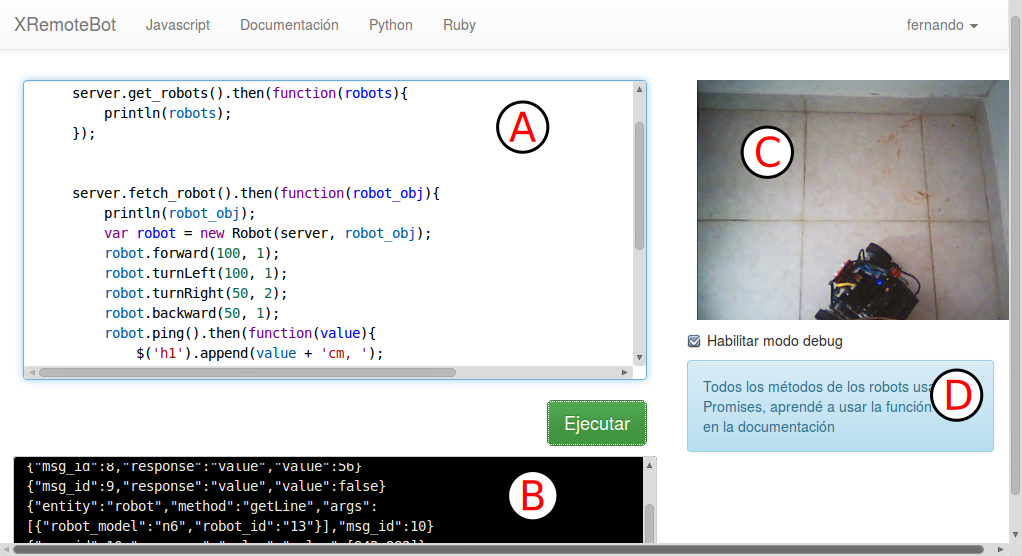
\includegraphics[width=1\textwidth]{figures/xremotebot_gui}
    \end{subfigure}\hskip 0.5em%
    \begin{subfigure}[m]{0.4\textwidth}
        \begin{description}
            \item[A:] área de texto para codificar.
            \item[B:] área que simula una consola. Los programas
                puedan imprimir texto en este área.
            \item[C:] transmisión
                de video. Muestra los robots en tiempo real.
            \item[D:] caja de ``tips'' o consejos.
        \end{description}
    \end{subfigure}
    \caption{Interfaz web de XRemoteBot}
    \label{fig:interfaz_web}
\end{figure}

Esta interfaz provee un sistema para crear usuarios nuevos, obtener las
API key y acceso a la documentación básica para trabajar con XRemoteBot
desde cualquiera de los tres clientes implementados.

La interfaz web fue pensada principalmente para ser utilizada en conjunto
 con el cliente
Javascript, aunque puede ser accedida sin problemas aún si se usa
otro de los clientes para poder visualizar los robots a través del
streaming de video. Provee un área de texto para escribir los scripts a
ejecutar.
Esta área de texto es creada con
CodeMirror\footnote{\url{https://codemirror.net/}}
que provee resaltado de sintaxis y manejo de los eventos de teclado para
que, al presionar \textit{Tab}, el editor indente el código en lugar de saltar a otro
elemento de la página como harían los navegadores por defecto.

Otra área de texto en la parte inferior
simula la salida de una terminal, en la misma
se pueden ver mensajes de log generados con la función
\texttt{rblog} que pueden ser habilitados o deshabilitados con la opción
``habilitar modo debug''
 y mensajes impresos con la función \texttt{println}.
Ambas funciones pueden imprimir, además de cadenas de texto, objetos. Estos últimos
se convierten a cadenas de texto usando la función \texttt{JSON.stringify()}.

Un área de video destinada a emisiones en vivo que muestren la posición
del robot, el mismo no requiere ningún plugin ya que se utilizó
\texttt{jsmpeg}\footnote{\url{https://github.com/phoboslab/jsmpeg}}
que permite emitir video en vivo usando WebSockets y renderizarlo
en el navegador en un elemento Canvas, de esta manera se logró tener
video en vivo utilizando características estándar de HTML5.

\appendix
% Apéndice A Serialización

\chapter{Serialización}
\label{ch:serializacion}

Siendo una aplicación cliente-servidor remotebot requiere algún método de
serialización para intercambiar datos entre los clientes y el servidor,
considerando que el servidor no es más que un servidor web que usa websockets
como protocolo, el método de serialización más adecuado parece ser JSON
(Javascript Serialization Object Notation).

JSON cuenta con las siguientes características:

\begin{enumerate}
    \item Está estandarizado (ECMA-404 http://www.ecma-international.org/publications/files/ECMA-ST/ECMA-404.pdf)
        y (rfc http://tools.ietf.org/html/rfc7159) el último es una propuesta de estándar (http://www.rfc-editor.org/info/rfc7159)
    \item Soporta los tipos de datos necesarios para intercambiar mensajes con
        los datos necesarios para controlar los robots usando un nivel de
        abstracción adecuado.
    \item Al ser un formato de texto es simple analizar el tráfico entre los
        clientes y el servidor para detectar posibles errores.
    \item Está soportado de forma nativa por los navegadores más utilizados
        (http://caniuse.com/#search=json).
\end{enumerate}

Pero también existen otras alternativas cuyos objetivos son serialización
y desserialización rápida, y datos serializados más compactos
como BSON (Binary JSON) y (CBOR Concise Binary Object Representation).

Algunas características de BSON y CBOR son:

\begin{enumerate}
    \item Codifican la información en formato binario.
    \item Son tan fáciles de usar como JSON.
    \item Ambos formatos proveen un superset de los tipos de datos provistos
        por JSON.
    \item CBOR tiene una especificación propuestas como estándar (CBOR http://tools.ietf.org/html/rfc7049)
    \item BSON tiene una especificación y una implementación bien conocida en MongoDB
    \item Por estar en formato binario decodificar una captura de tráfico
        para depurar un programa es más laborioso.
    \item En algunos casos estos formatos binarios generarán mensajes más
        chicos que JSON, pero no siempre.
    \item Requieren usar librerías Javascript en los clientes web ya que los
        navegadores no lo implementan de forma nativa.
\end{enumerate}

Para tomar un decisión respecto al formato a utilizar se decidió generar
16 archivos \texttt{JSON} con datos aleatorios, estos archivos se cargaron
con una cantidad de entradas múltiplo de 1024 desde 1024 hasta 16384, donde
cada una de estas entradas es un objeto \texttt{JSON} con 5 entradas de tipo
numérico, 5 strings, 5 objetos (cada uno con una entrada numérica) y 5
arrays (cada uno con 2 entradas de tipo string).

Estos archivos se cargaron desde scripts similares en Python y Javascript que
desserializaron y serializaron estos datos repetidas veces calculando el tiempo
promedio que llevó hacer cada una de estas acciones para cada formato.

Se eligió hacer las pruebas con Python y Javascript porque el primero es el
lenguaje de implementación del servidor y del cliente que probablemente tenga
más uso en un futuro, mientras que Javascript es el lenguaje de implementación
del cliente que se ejecutará en los navegadores web y que puede servir como
base para implementaciones con Brython, Skulp, Opal, etc...

Para hacer el experimento repetible y automatizable la implementación en
Javascript se ejecutó con el intérprete \textbf{nodejs} basado en
el motor \textbf{v8} usado por \textbf{Chrome} y además se crearon
scripts de apoyo para generar los datos de prueba, ejecutar los scripts
con los distintos formatos de forma automatizada y formatear los datos
resultantes en archivos csv.

Todas las pruebas se realizaron sobre Lihuen 6 beta (basado en Debian Jessie)
en una notebook con procesador ``Intel(R) Core(TM) i3 CPU M 370 @ 2.40GHz''
y 4GB de RAM % NOTA: son 4GB no 4GiB
usando Python 3.4.2 y NodeJS 0.10.35 (ya que la versión 0.10.29 distribuida al
momento con Debian Jessie tenía un bug que generaba un error de memoria al
desserializar strings largos con \texttt{JSON.load}~%
\footnote{\url{https://security-tracker.debian.org/tracker/CVE-2014-5256}}).

De estas pruebas se desprenden las mediciones de las figuras%
\ref{fig:ser-time-py}, \ref{fig:ser-time-js} y \ref{fig:ser-size}.

\begin{figure}

    \caption{Cantidad de entradas versus tiempo de serialización y desserialización en Python}
    \label{fig:ser-time-py}
\end{figure}

\begin{figure}

    \caption{Cantidad de entradas versus tiempo de serialización y desserialización en Javascript (nodejs)}
    \label{fig:ser-time-js}
\end{figure}

\begin{figure}

    \caption{Cantidad de entradas versus tamaño del archivo serializado}
    \label{fig:ser-size}
\end{figure}


\chapter{WebSockets y Promises}\label{cha:websockets_y_promises}

Para el desarrollo de este trabajo decidió utilizar dos tecnologías
que aún están en proceso de estandarización pero ya son ampliamente
soportadas por distintos navegadores
Web%
~\footnote{\url{http://caniuse.com/\#feat=websockets}}%
~\footnote{\url{http://caniuse.com/\#feat=promises}}
como son la API
\textit{WebSocket}~\footnote{La API en proceso de estandarización por la W3C,
pero el protocolo ya fue estandarizado por IETF.}
y la API \textit{Promise}~\footnote{En proceso de estandarización para
ECMAScript 6 (Harmony).}.

En este capítulo se presenta una breve reseña de ambos y los motivos
por los cuales fueron elegidos.

\section{WebSockets}

Para permitir el uso remoto de los robots a través de Internet sin necesidad
de requerir configuraciones ni puertos especiales se eligió implementar el
sistema como una
aplicación web. Sin embargo, como se menciona en el
capítulo~\ref{cha:serializacion} no se utiliza HTTP para el intercambio de
mensajes y valores de retorno entre los clientes y el servidor sino el
protocolo WebSocket.

El protocolo WebSocket permite mantener conexiones persistentes y no envía
encabezados HTTP en cada mensaje, reduciendo así el overhead en los mensajes
intercambiados que supondría el uso de HTTP~\citep{wang_2013}, aprovechando al
mismo tiempo los puertos TCP que abre el servidor Web.

La elección de este protocolo trae como desventaja frente al uso de HTTP la
necesidad de tener consideraciones de seguridad especiales, para la parte
Web del sistema se utiliza autenticación con cookies pero no resulta seguro
utilizar el mismo mecanismo para la sesión con WebSockets ya que el sistema
quedaría vulnerable a ataques de tipo CSRF (Cross-Site Request
Forgery)~\citep{owasp_2014}~\footnote{
\url{https://www.owasp.org/images/5/52/OWASP_Testing_Guide_v4.pdf}}.

Una de las estrategias recomendadas es verificar el encabezado \texttt{Origin}
desde el servidor, pero esta técnica no es suficiente ya que los
clientes pueden falsear este campo y solamente si el cliente es un navegador
envía este encabezado.
Otra estrategia es tener un mecanismo de autenticación
separado para la comunicación~\footnote{\url{https://www.christian-schneider.net/CrossSiteWebSocketHijacking.html}},
esta fue la estrategia elegida para XRemoteBot usando una \textit{API key}
para identificar a los usuarios al inicio de la comunicación.

\section{Promises}

La API de WebSockets disponible en los navegadores Web requieren
redefinir una serie de funciones de la instancia del WebSocket
para recibir y enviar mensajes~\citep{websocket_2014}, a saber:
\begin{description}
    \item[\texttt{WebSocket\#onopen()}] se ejecutará cuando
    la conexión esté establecida.
    \item[\texttt{WebSocket\#onerror()}] se ejecutará ante un error en
    la conexión.
    \item[\texttt{WebSocket\#onclose()}] se ejecutará si la conexión
    se cierra.
    \item[\texttt{WebSocket\#onmessage()}] se ejecutará al recibir un
    mensaje desde el servidor, recibe como argumento el mensaje
    enviado por el servidor.
\end{description}

La intención del autor es ocultar estos detalles de implementación de
los usuarios que quieran controlar los robots usando la API Javascript,
para esto es posible utilizar el objeto \textit{Promise} que se encuentra
en proceso de estandarización para ECMAScript 6, pero ya se puede
usar en los navegadores más populares.

Los objetos \textit{Promise} se utilizan para obtener valores resultantes
de cómputos asincrónicos, como es el caso de la respuesta a una petición
hecha con WebSockets, la interfaz de \textit{Promise} no permite programar
los robots en Javascript con una interfaz idéntica a la usada al programar
los robots con la biblioteca DuinoBot, pero es relativamente fácil de
utilizar y ante la imposibilidad de demorar la ejecución del código
Javascript sin crear funciones adicionales provee una alternativa
relativamente simple en comparación con el uso directo de la interfaz
de los objetos \texttt{WebSocket}.

Los objetos \textit{Promise} se instancian pasándoles como argumento una
función que a su vez recibe 2 argumentos, \texttt{resolve} y \texttt{reject}.
El primer argumento ``cumple'' o ``resuelve'' la promesa y el segundo la
``rechaza''.
Las ``promesas'' tienen dos métodos: \texttt{then} y \texttt{catch} que se
ejecutan cuando la promesa se ``cumple'' o se ``rechaza'' respectivamente.

XRemoteBot para Javascript al crear cada mensaje le asigna un \texttt{msg\_id},
crea una \texttt{Promise} y guarda en un \texttt{object} de mensajes
pendientes un objeto que contiene las funciones \texttt{resolve} y
\texttt{reject} asociados con esa \texttt{Promise}
usando como clave el \texttt{msg\_id}. Al recibir una respuesta
desde el servidor, el cuerpo de \texttt{WebSocket\#onmessage()} toma el
\texttt{msg\_id} de la respuesta, lo utiliza para recuperar las funciones
asociadas con la \texttt{Promise} de este mensaje y ejecuta el
\texttt{resolve} pasándole como argumento la respuesta del servidor.
De esta manera las ``promesas'' asociadas con cada
mensaje se ``cumplen'' al obtener la respuesta correspondiente del servidor.

Cada método de XRemoteBot para Javascript que involucre enviar un mensaje
retornará una ``promesa'' que se cumplirá cuando el servidor responda
el mensaje.

Esto permite, por ejemplo, obtener el valor del sensor de distancia de un 
robot de forma simple como se ve en el código~\ref{lst:promises_get_obstacle}.
Si bien esta interfaz no es idéntica a la de DuinoBot, es lo más parecido
que se pudo lograr.

\begin{lstlisting}[language=C,
caption={Implementación de \texttt{getObstacle()} con ``promesas''},
label=lst:promises_get_obstacle]
robot.getObstacle().then(function(hay_obstaculo){
    if (hay_obstaculo.value){
        console.log("Hay un obstáculo al frente");
    }
    else {
        console.log("No hay obstáculos");
    }
});
\end{lstlisting}

\include{biblio}
\end{document}

